\documentclass[a4paper]{scrartcl}

% Localization
\usepackage[english]{babel}
\usepackage[T1]{fontenc}
\usepackage[utf8]{inputenc}

% Quotations
\usepackage{dirtytalk}

% PDF-compatible landscape mode
\usepackage{pdflscape}

% Advanced tables
\usepackage{array}
\usepackage{tabularx}

% Fancy tablerules
\usepackage{booktabs}

% Graphics
\usepackage{caption}
\usepackage{subcaption}
\usepackage{graphicx}
\graphicspath{{resources}}

% Decent quotations
\usepackage{csquotes}

% Automatic float barriers to each \section
% \usepackage[section]{placeins}

% Math
\usepackage{amssymb,amsmath,amsfonts}
\usepackage{mathtools}

% Algorithms
\usepackage{algpseudocode}
% And floats for it
\usepackage{algorithm}

% Multi column support
\usepackage{multicol}

% SI units
\usepackage[binary-units]{siunitx}

% Clickable links in PDF
\usepackage{hyperref}

\newcommand{\rgets}{\overset{\mathrm{R}}{\gets}}
\newcommand{\setbin}{\{0, 1\}}

\title{41106 - Cryptographic Protocols}
\subtitle{Summary}
\author{Michael Senn}
\date{\today}

\begin{document}

\maketitle % Inserts the title, author and date

\tableofcontents

\begin{abstract}
		This summary is based on the lecture notes and slides. It was created
		for the sole purpose of preparing for an exam, with no focus on
		proof-reading, a coherent structure or being suitable for other people.
		Use at your own discretion.
\end{abstract}

\section{Introduction}

Topics:
\begin{itemize}
		\item Computing with encrypted data
		\item Authenticating without revealing information
		\item Voting
		\item ...
\end{itemize}

\subsection{Example: Generating a random bit among two parties}

\begin{algorithm}
		\caption{Random coin flip among two parties}
		\begin{multicols}{3}
				\begin{algorithmic}[0]
						\State \textbf{A}
						\State $a \rgets \setbin$
						\State $x \rgets \setbin^k$
						\State $c \coloneqq H(a || x)$
						\State
						\State \textbf{Verify} $d = H(b || y)$
						\State \textbf{Return} $a \oplus b$
				\end{algorithmic}

				\columnbreak

				\begin{algorithmic}[0]
						\State 
						\State 
						\State 
						\State $\xleftrightarrow{c, d}$
						\State $\xrightarrow{a, x}$
						\State $\xleftarrow{b, y}$
				\end{algorithmic}

				\columnbreak

				\begin{algorithmic}[0]
						\State \textbf{B}
						\State $b \rgets \setbin$
						\State $y \rgets \setbin^k$
						\State $d \coloneqq H(b || y)$
						\State \textbf{Verify} $c = H(a || x)$
						\State
						\State \textbf{Return} $a \oplus b$
				\end{algorithmic}
		\end{multicols}
\end{algorithm}

\begin{description}
		\item[Security] $c$ reveals nothing about $a$, so $B$ cannot bias $b$.
				As $A$ cannot construct a hash conflict, $A$ can also not
				change its value. As long as one party is honest, the resulting
				bit will be uniform.
\end{description}

\subsection{Example: Voting between parties}

Given parties $p_i$ with votes $v_i$, $i \in \{1, 2, 3\}$, calculate $\sum v_i$
confidentially. Protocol for $p_i$:
\begin{itemize}
		\item $x_{i,1}, x_{i, 2}, x_{i, 3} \coloneqq share(v_i)$, where $share$
				st $\sum x_{i, j} = v_i \mod p$
		\item Send $x_{i,j}$ to $p_j$, receive $x_{j, i}$ from $p_j$
		\item $y_i \coloneqq (x_{1, i} + x_{2, i} x_{3, i} \mod p$
		\item Send $y_i$ to all $p_j$, receive $y_j$ from $p_j$ where $j \neq i$
		\item Output $(y_1 + y_2 + y_3) \mod p$
\end{itemize}

\begin{description}
		\item[Privacy] Sharing of votes hides details from every party
		\item[Completness] Follows directly from choice of shares and algebra
\end{description}

\subsection{Goals}

\begin{description}
		\item[Privacy] No party larns more information than the output --- as
				if it was computed by a trusted party $T$.
		\item[Correctness] Every party receives the correct output. If there is
				a faulty input, the output is still consistent for all correct
				parties.
		\item[Input independence] Inputs of faulty parties must not depend on
				inputs of correct parties.
		\item[Fairness] Faulty parties receive output if and only if correct
				parties receive output.
\end{description}

\subsection{Fault types}

\begin{description}
		\item[Semi-honest] Faulty parties execute protocol correctly, but leak
				all internal values to adversary.
		\item[Malicious] Faulty parties behave arbitrarily, act against correct
				parties in a coordinated manner.
\end{description}


\section{Basic techniques}

\subsection{Programs as circuits}

Idea: Every program on inputs $x_1, \ldots x_n$ computes function $f(x_1,
\ldots x_n)$ which can be represented by a turing machine or a circuit.

\subsubsection{Cook-Levin theorem}

Every problem decideable by a non-deterministic turing machine in polynomial
tmie can be formulated as the SAT of a polynomial-size circuit.

\subsection{Public-key cryptography}

\subsubsection{Discrete logarithms}

Given $G = <g>$, the discrete log of $y \in G$ is $i$ such that $g^i = y$.

\paragraph{DLP}

Given $y = g^x$ for $x \in \mathbb{Z}_q$, find $x$.

\paragraph{CDH}

Given $x = g^a, y = g^b$ for $a, b \in \mathbb{Z}_q$, compute $g^{a \cdot b}$.

\paragraph{DDH}

Given $x = g^a, y = g^b, z = g^c$, where $c$ is either $ab$ or a random value
in $\mathbb{Z}_q$, differentiate the two cases.

\subsubsection{Public-key encryption formalization}

\begin{description}
		\item[Completness] $Dec(sk, Enc(pk, m)) = m \forall m$
		\item[Security] An encryption of any $m$ is indistinguishable from a random
				element of the ciphertext space. For two messages $m_1, m_2$ no
				adversary can distinguish $Enc(pk, m_1)$ from $Enc(pk, m_2)$.
\end{description}

\subsubsection{RSA Correctness}

Uses Fermat's little theorem, given $p$ prime, $a$ integer, $a, p$ coprime:
\begin{align*}
		a^{p-1} \equiv 1 \mod p
\end{align*}

And statement from CRT:
\begin{align*}
		a \equiv b \mod pq \Leftrightarrow a \equiv b \mod p \land a \equiv b \mod q
\end{align*}

Further:
\begin{align*}
		\phi(N) = (p - 1)(q - 1) \Rightarrow (p - 1) | \phi(N) \land (q - 1) | \phi(N)
\end{align*}

Then either $m \equiv 0 \mod p$ in which case $m^{ed} \equiv 0 \mod p$
directly, or:
\begin{align*}
		m^{ed} \equiv m^{ed - 1} \cdot m \equiv m^{(p-1)^h} \cdot m \equiv 1^h \cdot m \equiv m \mod p
\end{align*}

Equivalently for $\mod q$.


\subsection{Digital signatures}

\subsubsection{RSA}

Naive implementation using $Sign(sk, m) = m^d \mod N$ insecure, as adversary
could pick arbitrary $\sigma*, m := \sigma*^e$, which would pass verification.
Instead use hashed RSA signatures, `signing' $H(m)$ instead of $m$ directly.

\section{Blind signatures}

Goal: Protocol to allow $A$ to get $B$'s signature on $m$ without $B$ learning
the message, nor being able to associate a later signature with this action.
Compare: Signing envelope.

\subsection{Blind signatures for RSA}

Key generation as in RSA.

\begin{algorithm}
		\caption{Blind RSA signatures}
		\begin{algorithmic}[0]
				\Procedure{Sign}{$sk, m$}
				\State \textbf{A}
				\State $r \rgets \mathbb{Z}_N$
				\State $h' \coloneqq H(m) \cdot r^e \mod N$
				\State $h' \rightarrow B$
				\State \textbf{B}
				\State $s' \coloneqq h'^d \mod N$
				\State $A \leftarrow s'$
				\State \textbf{A}
				\State $s \coloneqq s' / r$
				\EndProcedure

				\Procedure{Verify}{$pk, m, s$}
				\State $s^e == H(m)$
				\EndProcedure
		\end{algorithmic}
\end{algorithm}

\subsection{Schnorr signatures (non-blind)}

Defined over $q$-order subgroup $G$ of $\mathbb{Z}^*_p$, with $p = m \cdot q +
1$.

\begin{algorithm}
		\caption{Schnorr signatures}
		\begin{algorithmic}[0]
				\Procedure{KeyGen}{}
				\State $x \rgets \mathbb{Z}_q$
				\State $Y \coloneqq g^x$
				\State \textbf{Return} $(Y, x)$
				\EndProcedure

				\Procedure{Sign}{$x, m$}
				\State $r \rgets \mathbb{Z}_q$
				\State $R \coloneqq g^r$
				\State $c \coloneqq H(m || t)$
				\State $s \coloneqq r - c \cdot x$
				\State \textbf{Return} $(c, s)$
				\EndProcedure

				\Procedure{Verify}{$Y, m, (c, s)$}
				\State \textbf{Return} $c == H(m || g^s \cdot Y^c)$
				\EndProcedure
		\end{algorithmic}
\end{algorithm}

\subsection{Blind schnorr signature scheme}

Key gen and verify same as in original.

\begin{algorithm}
		\caption{Blind Schnorr signatures}
		\begin{algorithmic}[0]
				\Procedure{Sign}{$x, m$}
				\State \textbf{B}
				\State $r \rgets \mathbb{Z}_q$
				\State $R \coloneqq g^r$
				\State $A \leftarrow R$

				\State \textbf{A}
				\State $\alpha, \beta \rgets \mathbb{Z}_q$
				\State $R' \coloneqq R \cdot g^{-\alpha} \cdot y^{-\beta}$
				\State $c' \coloneqq H(m || R')$
				\State $c \coloneqq c' + \beta$
				\State $c \rightarrow B$

				\State \textbf{B}
				\State $s \coloneqq r - c \cdot x$
				\State $A \leftarrow s$

				\State \textbf{A}
				\State $s' \coloneqq s - \alpha$
				\State \textbf{Return} $(c', s')$
				\EndProcedure
		\end{algorithmic}
\end{algorithm}

\subsection{Anonymous digital cash}

Given user $A$, shop $S$, bank $B$. Bank creates coins and stores balances, $A$
wants to exchange coins for services at $S$.

Goals:
\begin{itemize}
		\item If $A$ withdraws from $B$, then $B$ debits it from balance of $A$
		\item If $A$ transfers to $S$, then $B$ will credit coin to balance of $S$
		\item $B$ does not credit a coin to $S$ unless $B$ has issued the coin
				to some valid user $X$, and $X$ has transferred it to $S$
		\item If $B$ credits a coin to $Y$, then $B$ cannot link this coin to
				any withdrawal of a user.
\end{itemize}

\subsubsection{Protocol}

\begin{itemize}
		\item When $A$ wants to withdaw $u$ coins, it generates a random
				identifier $m$, blinds it as $m'$, and gets $B$ to issue a
				blind signature on $m'$. $B$ lowers $A$'s balance by $u$ and
				issues it a signature $\sigma'$ on $m'$. $A$ unblinds the
				signature to $\sigma$ and stores $(u, m, \sigma)$ in its
				wallet.
		\item To spend a coin, $A$ sends $(u, m, \sigma)$ to $S$. $S$ deposits
				it in the bank. If successful, it delivers goods or services to
				$A$.
		\item To deposit a coin, the bank verifies that $\sigma)$ is a valid
				signature for $m$. It also checks that $m$ was not yet in its
				list of already spent coins, and adds it to said list. If all
				is well, it increases the balance of $S$.
\end{itemize}


\section{Homomorphic encryption}

Goal: Compute on encrypted data with no interaction between user and cloud.

\subsection{Single homomorphic encryption}

Encryption scheme supporting operation $\oplus$ such that $Enc(x) \oplus Enc(y)
= Enc(x + y)$, or operation $\otimes$ such that $Enc(x) \otimes Enc(y) = Enc(x
\cdot y)$, where $x, y$ from some finite field of prime order.

Examples: Additively homomorphic ElGamal.

\subsection{Multiplicatively homomorphic ElGamal}

Textbook ElGamal is already multiplicatively homomorphic. Let $(R, C) = (g^r, m
\cdot y^r), (R', C') = (g^{r'}, m \cdot y^{r'})$ be two ciphertexts. Then the
component-wise multiplication $(\hat{R}, \hat{C}) = (g^{r + r'}, m \cdot m'
\cdot y^{r + r'})$ is a valid encryption of $m \cdot m'$.

\subsubsection{Additively homomorphic ElGamal}

Using $Enc$ and $Dec$ of textbook ElGamal, let:

\begin{algorithm}
		\caption{AM-ElGamal}
		\begin{algorithmic}[0]
				\Procedure{AM-Enc}{$y, m$}
						\State \textbf{Return} $\operatorname{Enc}(y, g^m)$
				\EndProcedure

				\Procedure{AM-Dec}{$x, (R, C)$}
						\State $h \coloneqq \operatorname{Dec}(x, (R, C))$
						\For{$i \gets 0, max$}
								\If{$g^i = h$}
										\State \textbf{Return} $i$
								\EndIf
						\EndFor
						\State \textbf{Return} error
				\EndProcedure
		\end{algorithmic}
\end{algorithm}

\subsection{Voting protocol using AM ElGamal}

\begin{itemize}
		\item Parties $P_i$ with votes $v_i$, authority $A$
		\item $A$ generates keypair, distributes public key
		\item $A$ computes $c_0 = \operatorname{Enc}(pk, 0)$ and sends to $P_1$
		\item $P_i$ computes $c_i = c_{i-1} \oplus Enc(y, v_i)$ and sends to
				$P_{i+1}$ ($P_n$ sends to $A$)
		\item $A$ decrypts $z = \operatorname{Dec}(x, c_n)$
		\item $A$ publishes $z = \sum_{i = 1}^n v_i$
\end{itemize}

Note:
\begin{itemize}
		\item Not robust against malicious parties. They can encrypt values
				other than $0, 1$, refuse to send the ciphertext on (or send
				malicious values), or $A$ can refuse to decrypt.
		\item Defenses: ZKP to prove valid vote, public bulletin board for
				communciation, distributed implementation of $A$ using secret
				sharing.
\end{itemize}

\section{Zero-knowledge proofs}

Prove statement is true, or knowledge of information, without giving away any
more information. Two kinds:

\begin{description}
		\item[Proof for statement] E.g. given boolean formula, there exists a
				set of variables such that it evaluates to true. Given two
				graphs, they are isomorph. Given a graph, there exists a
				hamiltonian circuit.
		\item[Proof of knowledge] Given $y$, I know $x$ such that $y = g^x$.
				Given a binary string $h$, I know $x$ such that $H(x) = h$.
				Given $n$ I know $p, q$ such that $n = pq$.
\end{description}

Requirements:
\begin{description}
		\item[Completness] If $S$ holds, prover $P$ correct, verifier $V$
				correct, then $V$ accepts.
		\item[Soundness] If $S$ false, then honest verifier $V$ will reject
				with at least a constant non-zero probability.
		\item[Zero-knowledge] $V$ learns only that $S$ holds, and not more.
\end{description}

For proof, show that:
\begin{description}
		\item[Completness] It holds with $P, V$ honest
		\item[Soundness] Given $P$ malicious, $V$ will reject with at least
				constant non-zero probability.
		\item[Zero knowledge] $V$ can also generate output with same
				distribution as protocol on its own (if in different order).
\end{description}

\subsection{Graph isomorphism}

$P$, $V$ given two graphs $G_0 = (V, E_0), G_1 = (V, E_1)$. $P$ knows an
isomorphism $f$ between the two, i.e. a bijective $f: V \rightarrow V$ such that
$\forall v, w \in V: (v, w) \in E_0 \Leftrightarrow (f(v), f(w)) \in E_1$.

\subsubsection{Protocol}

\begin{enumerate}
		\item $P$ chooses random permutation $\Pi$ on $V$, computes $H = (V,
				F)$ such that $H$ is isomorphic to $G_0$. Sends $H$ to $V$.
		\item $V$ sends random bit $b$
		\item $P$ shows isomorphism $\rho = \Pi$ for $b = 0$, $\rho = \pi \circ
				f^{-1}$ for $b = 1$.
		\item $V$ checks if $G_b$ is isomorphic to $H$.
\end{enumerate}


\subsection{What can be proven in zero-knowledge}

\begin{itemize}
		\item Graph isomorphism ($\not \in P$, believed to be between $P$ and
				$NP$)
		\item If one NP-complete problem has a ZKP, any NP-complete problem has
				a ZKP (polynomial time)
		\item 3-Colourability of a graph $G$ is NP-complete nad has ZKP
		\item In theorey: Can be used for online authentication. In practice:
				Not used, as more efficient schemes exist.
\end{itemize}

\subsection{Zero-knowledge proof of knowledge}

Goal: Prove knowledge of $\alpha, \beta, \ldots$ such that $\Phi(\alpha, \beta,
\ldots)$ holds. Example: Prove knowledge of $\alpha$ such that $g^\alpha = y$.

Notation: $PK\{(\alpha, \beta, \ldots) : \Phi(\alpha, \beta, \ldots)\}$. E.g.
$PK\{(\alpha) : y = g^\alpha\}$.

\subsubsection{Formalization}

Three stages:
\begin{itemize}
		\item Commitment $t$ from $P$ to $V$
		\item Challenge $c$ from $V$ to $P$
		\item Response $s$ from $P$ to $V$
		\item $V$ verifies response
\end{itemize}

Properties: Similar to ZKP.
\begin{description}
		\item[Completness] If $P$ has input $x$ such that $\Phi(x)$ holds, then
				$V$ accepts
		\item[Soundness] Given two accepting transcripts $(t, c, s), (t, c',
				s'), c \neq c'$ and $\Phi(x)$, there is an efficient knowledge
				extractor $E$.
		\item[Zero-knowledge] $V$ can simulate transcripts $(t, c, s)$ on its
				own with indistinguishable distribution.
\end{description}

\subsection{ZKPK of discrete log}

\begin{algorithm}
		\caption{ZKPK of discrete log}

		\begin{multicols}{2}
				\begin{algorithmic}[0]
						\State \textbf{A}
						\State $r \rgets \mathbb{Z}_q$
						\State $t \coloneqq g^r \rightarrow$
						\State
						\State $s \coloneqq r - x \cdot c \rightarrow$
				\end{algorithmic}

		\columnbreak

				\begin{algorithmic}[0]
						\State \textbf{B}
						\State
						\State
						\State $\leftarrow c \rgets \mathbb{Z}_q$
						\State \textbf{Verify} $g^s \cdot y^c = t$
				\end{algorithmic}
		\end{multicols}
\end{algorithm}

\subsection{Commitment schemes}

Set of primitives between receiver $R$ and sender $S$.

Three algorithms:
\begin{description}
		\item[$KeyGen() \rightarrow pk$] Probabilistic, outputs public key
		\item[$Com(pk, x, r) \rightarrow c$] Outputs commitment $c$ as bit
				string to $x$. Probabilistic, $r$ introduces randomness.
		\item[$Ver(pk, x, r, c) \rightarrow TRUE / FALSE$] Deterministic,
				returns whether $r$ and $x$ correctly `open' commitment $c$.
\end{description}

Properties:
\begin{description}
		\item[Completness] For $pk \coloneqq KeyGen(), x \in \{0, 1\}^*, r \in
				R: Ver(pk, x, r, Com(pk, x, r)) = True$
		\item[Unconditional binding] Security for $R$ against $S$. No $S'$ can produce $(x,
				r), (x', r')$ with $x \neq x'$ which both pass verification.
				\begin{itemize}
						\item Optionally: Weaker version for only
								computationally bounded adversaries, which
								cannot do so except with neglibible
								probability.
				\end{itemize}
		\item[Unconditional hiding] Security for $S$ against $R$. For any two
				commitments to different values, no $R$ can guess --- given a
				single commitment --- which value the commitment is for with $p
				> 1/2$.
				\begin{itemize}
						\item Optionally: Weaker version for computationlly
								bounded aversaries, which can guess with
								probability at most $p > 1/2 + \sigma$ for a
								negligible $\sigma$.
				\end{itemize}
\end{description}


\subsection{ZKPK of representation}

Proof knowledge of $\alpha_i$ such that $y = \prod g_i^{\alpha_i}$:

\[
		PK\{ (\alpha_1, \alpha_2, \ldots, \alpha_n) : y = g_1^{\alpha_1} \cdot \ldots \cdot g_n^{\alpha_n} \}
\]

Where the DL base $g_i$ of $g_j$ is unknown for all $i \neq j$.

\begin{algorithm}
		\caption{ZKPK of representation}

		\begin{multicols}{2}
				\begin{algorithmic}[0]
						\State \textbf{A}
						\State $r_i \rgets \mathbb{Z}_q$
						\State $t \coloneqq \prod g_i^{r_i} \rightarrow$
						\State
						\State $s_i \coloneqq r_i - c \cdot \alpha_i \rightarrow$
				\end{algorithmic}

				\columnbreak

				\begin{algorithmic}[0]
						\State \textbf{B}
						\State
						\State
						\State $\leftarrow c \rgets \mathbb{Z}_q$
						\State \textbf{Verify} $t = (\prod g_i^{s_i}) \cdot y^c$
				\end{algorithmic}
		\end{multicols}
\end{algorithm}

Applicability: Prove knowledge of plaintext $m$ of additively homomorphic
ElGamal ciphertext $(R, C) = (g^r, g^m \cdot y^r)$: $C = g^m \cdot y^r$.

\subsection{Proof of equality}

Proof that $DL_{g_1}(y_1) = DL_{g_2}(y_2)$:

\[
		PK\{ (\alpha) : y_1 = g_1^\alpha \land y_2 = g_2^\alpha \}
\]

\begin{algorithm}
		\caption{ZKPK of equality}

		\begin{multicols}{2}
				\begin{algorithmic}[0]
						\State \textbf{A}
						\State $r \rgets \mathbb{Z}_q$
						\State $t_i \coloneqq g_i^r \rightarrow$
						\State
						\State $s \coloneqq r - c \cdot x \rightarrow$
				\end{algorithmic}

				\columnbreak

				\begin{algorithmic}[0]
						\State \textbf{B}
						\State
						\State
						\State $\leftarrow c \rgets \mathbb{Z}_q$
						\State
						\State \textbf{Verify} $t_i = g_i^s \cdot y_i^c$
				\end{algorithmic}
		\end{multicols}
\end{algorithm}

Applicability: Prove that additively homomorphic ElGamal ciphertext $(R, C) =
(g^r, g^m \cdot y^r)$ is a valid encryption of $m \in \{0, 1\}$ by combining
with proof of disjunction: $\log_g(R) = \log_y(C / g^0) \lor \log_g(R) = \log_y(C / g^1)$

\subsection{Proof of conjunction (AND)}

Idea: Use same challenge in two parallel proofs.

\subsection{Proof of disjunction (OR)}

Assume $P$ only knows $x_b$, not $x_{b'}$. Wants to prove $PK\{ (x_1, x_2)
: \Phi_1(y_1, x_1) \lor \Phi_2(y_2, x_2) \}$.

\begin{algorithm}
		\caption{ZKPK of disjunction}

		\begin{multicols}{2}
				\begin{algorithmic}[0]
						\State \textbf{A}
						\State $(t_b, r_b) \coloneqq \operatorname{commit}(y_b)$
						\State Fake proof for $x_{b'}$
						\State $c_{b'} \coloneqq \operatorname{challenge}()$
						\State $(t_{b'}, r_{b'}, s_{b'}) \coloneqq \operatorname{simulate}(y_{b'}, c_{b'})$
						\State $\xrightarrow{t_0, t_1}$
						\State
						\State $c_b \coloneqq c + c_{b'}$
						\State $s_b \coloneqq \operatorname{response}(x_b, y_b, t_b, r_b, c_b)$
						\State $\xrightarrow{c_0, s_0, c_1, s_1}$
				\end{algorithmic}

				\columnbreak

				\begin{algorithmic}[0]
						\State \textbf{B}
						\State
						\State
						\State
						\State
						\State
						\State $\leftarrow c \coloneqq \operatorname{challenge}()$
						\State
						\State
						\State \textbf{Verify} $c_0 + c_1 = c \land \operatorname{verify}(y_1, y_1, c_1, s_1) \land \operatorname{verify}(y_2, t_2, c_2, s_2)$
				\end{algorithmic}
		\end{multicols}
\end{algorithm}

\subsection{Making ZKPK non-interactive}

Remove interactino by computing challenge $c$ using a one-way function from
$t$. Called `Fiat-Shamir transformation'.

Example from Schnorr proof:
\begin{enumerate}
		\item $c \coloneqq H(t || m)$. In this case $m$ added as some context
				of message $m$.
		\item Output simulated transcript $(t, s)$ of ZKPK
\end{enumerate}

\subsection{Discrete-log based commitments}

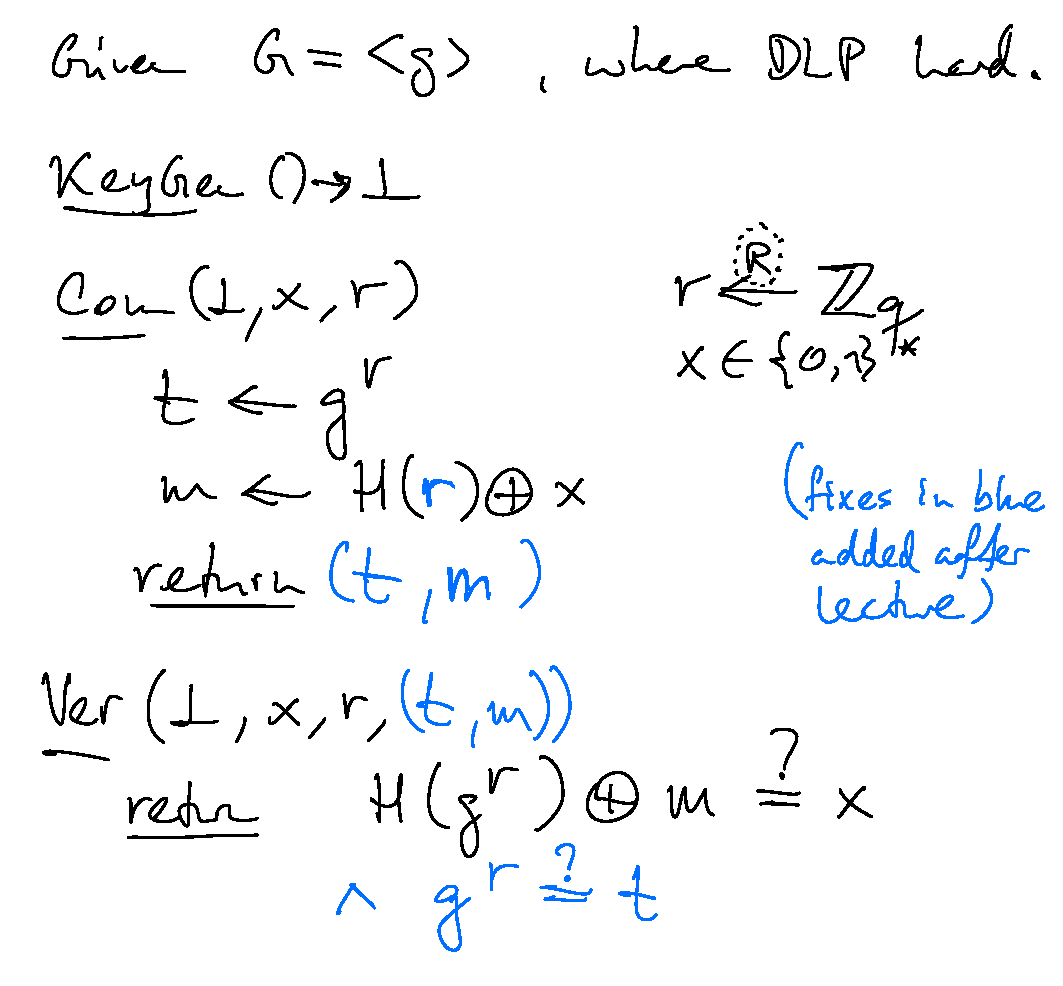
\includegraphics[width=\textwidth]{06_dl_commitments}

\subsection{Pedersen commitments}

Given $G = <g> = <h>$, $g, h$ generated independently (e.g. trusted setup).


\begin{algorithm}
		\caption{Pedersen-based commitment scheme}

		\begin{algorithmic}[0]
				\Procedure{KeyGen}{}
						\State $h \rgets G$
						\State \textbf{Return} $h$
				\EndProcedure

				\Procedure{Commit}{$h, x, r$}
						\State $r \rgets \mathbb{Z}_q$
						\State \textbf{Return} $g^x \cdot h^r$
				\EndProcedure

				\Procedure{Verify}(h, x, r, c)
						\State \textbf{Return} $c == g^x \cdot h^r$
				\EndProcedure
		\end{algorithmic}
\end{algorithm}

Information-theoretically unconditionally hiding. But need to convince all
parties that generators were computed correctly (i.e. independently).


\section{Oblivious two-party protocols}

\begin{description}
		\item[OPRF] Oblivious pseud-random function
		\item[PSI] Private set intersection
		\item[OT] Oblivious transfer]
\end{description}

\subsection{OPRF}

Recall PRF: $F : \{0, 1\}^\lambda \times \{0, 1\}^k \rightarrow \{1,
0\}^{out}$. $F(k, x)$ should `look random' to any party that does not know $k$.
In practice, PRF implemented as $F(k, x) \coloneqq HMAC(k, x)$.

Oblivious case: Sender $S$ provides $k$, receiver $R$ provides $x$.

\subsubsection{Properties}

\begin{itemize}
		\item As regular PRF: $R$ cannot distinguish $L^{OPRF}_{prf-real}$ from
				$L^{OPRF}_{prf-rand}$.
		\item Oblivious: For any two $x, x'$, $S$ cannot distinguish which one
				$R$ used as input to OPRF.
\end{itemize}


\subsubsection{Construction of PRF}

Given $G = <g>, |G| = q$, $H : \{0, 1\}^{in} \rightarrow G$, $I : \{0, 1\}^{*}
\rightarrow \{0, 1\}^{out}$ two hash functions, we construct a PRF $F:
\mathbb{Z}_q \times \{0, 1\}^{in} \rightarrow \{0, 1\}^{out}$ as follows:

\[
		F(k, x) \coloneqq I(H(x)^k)
\]

This is a PRF assuming hardness of CDH in the R.O.M.

\subsubsection{Oblivious evaluation of PRF $F$}

\begin{algorithm}
		\caption{Oblivious evaluation of PRF}

		\begin{multicols}{2}
				\begin{algorithmic}[0]
						\State \textbf{S}
						\State
						\State
						\State $w \coloneqq r^k \rightarrow$
				\end{algorithmic}

				\columnbreak

				\begin{algorithmic}[0]
						\State \textbf{R}
						\State $r \rgets \mathbb{Z}_q$
						\State $\leftarrow v \coloneqq H(x)^r$ \Comment{in G}
						\State
						\State $y \coloneqq J(w^{r^{-1}})$
				\end{algorithmic}
		\end{multicols}
\end{algorithm}

Security for $S$ holds also with malicious $R$, because it only sees a group
element. Security for $R$ holds for semi-honest $S$, a malicious $S$ could send
a $\hat{w} \neq w$. To fix this: E.g. ZKP.

\subsection{PSI}

$A$ holds set $X$, $B$ holds set $Y$. Goal: Calculate $X \cap Y$ in oblivious
way. Assume sets are represented as bit strings of some finite length.

\subsubsection{Insecure protocol}

\begin{enumerate}
		\item $A$ calculates $h_x \coloneqq H(x) \forall x \in X$, $B$
				calculates $h_y \coloneqq H(y) \forall y \in Y$
		\item $A$ sends $H_A$ the set of all hashes to $B$. $B$ intersects with
				the set of all hashes $H_B$
		\item $B$ calculates $Z = X \cap Y$, by checking for which $y \in Y$
				there is a hash value in $H_A \cup H_B$.
\end{enumerate}

This is insecure, as $B$ is able to test any element $z$ whether $H(z)$ is
contained in $H_A$.

\subsubsection{PSI using OPRF}

\begin{enumerate}
		\item $A$ picks OPRF key $k$
		\item $A$, $B$ transfer the PRF values of $y \in Y$, $H_B$ ($B$, acting
				as the recipient, learns them)
		\item $A$ sends PRF values of $x \in X$, $H_A$ (can compute them locally)
		\item $B$ computes intersection $Z = H_A \cap H_B$
		\item $B$ sends those $y \in Y$ for which there is an entry in $Z$
\end{enumerate}



\subsection{Oblivious transfer}

Sender $S$ holds $x_1, \ldots, x_n$. Receiver $R$ wants $x_c$, such that $S$
learns nothing of $c$, $R$ learns nothing of $x_{c'} with c' \neq c$.


\subsubsection{2-1 OT from ElGamal}


Idea: $R$ prepares two public keys, $y_0, y_1$, such that it knows the private
key of only $y_c$. Then $S$ can publish both ciphertexts $c_1, c_2$, and $R$
will be able to decrypt only $c_c$ to $x_c$.

\begin{algorithm}
		\caption{2-1 OT using ElGamal}

		\begin{multicols}{2}
				\begin{algorithmic}[0]
						\State \textbf{S}
						\State $r \rgets \mathbb{Z}_q$
						\State $t \coloneqq g^{r} \rightarrow$
						\State
						\State
						\State
						\State
						\If{$t \neq y_0 \cdot y_1$}
						\State \textbf{Halt}
						\EndIf
						\State $(R_0, C_0) \coloneqq Enc(y_0, x_0)$
						\State $(R_1, C_1) \coloneqq Enc(y_1, x_1)$
						\State $\xrightarrow{(R_0, C_0, R_1, C_1)}$
				\end{algorithmic}

				\columnbreak

				\begin{algorithmic}[0]
						\State \textbf{R}
						\State
						\State
						\State $x_c \rgets \mathbb{Z}_q$
						\State $y_c \coloneqq g^{x_c}$
						\State $y_{c'} \coloneqq \frac{t}{y_c}$
						\State $\xleftarrow{y_0, y_1}$
						\State
						\State
						\State
						\State
						\State
						\State \textbf{Return} $Dec(x_c, R_c, C_c)$
				\end{algorithmic}
		\end{multicols}
\end{algorithm}

Security for $S$ based on DL (so $R$ cannot know DL of both $y_0$ and $y_1$)
and security of ElGamal. Security for $R$ unconditional, as it only sends two
identically distributed values.

\section{Secure two-party computation (2PC)}

Goal: Evaluate $f(x, y)$ between parties $A$ and $B$, with $A$ holding $x$, $B$
holding $y$. One of them ($B$) should learn $f(x, y)$, and neither should learn
more of the other's input than $f(x, y)$ itself implies.

\subsection{Toy example using OT}

If domain of $y \in Y$ is small, $A$ prepares $s_y \coloneqq f(x, y) \forall y
\in Y$, and sends $\{s_y\}$ via $1-of-|Y|$ OT to B. $B$ selects output $y$, and
will thus learn $s_y = f(x, y)$ directly.

Issue in general: With $m$-bit input of $B$, the OT would have $2^m$ options.

\subsection{Towards Yao's garbled circuits construction}

Assume asymmetric encryption scheme which allows to check whether a key is the
correct key for a giphen ciphertext. $Dec(k, c)$ returns $\bot$ if $c$ was not
produced as $Enc(k, m)$ for some message $m$.

Can be implemented as e.g. authenticated encryption, or by appending a magic
bitstring to messages before encrypting them, which can be checked for after
decryption.

\subsubsection{Encrypt function table of $f$}

\begin{enumerate}
		\item Represent every $x \in X, y \in Y$ with a random key $k_x, k_y$ respectively.
		\item For $x \in X, y \in Y$ compute $f(x, y)$ and encrypt it in Table
				$T$ at position $T_{x, y}$: $T_{x, y} \coloneqq Enc(k_x \cdot
				k_y, f(x, y))$
		\item Transfer key $k_y$ (of B's input $y$) to $B$, send $k_x$ to B
		\item $B$ tries to decrypt all entries, and succeeds in $f(x, y)$
\end{enumerate}

\begin{algorithm}
		\caption{Encrypted function table of $f$}

		\begin{multicols}{2}
				\begin{algorithmic}[0]
						\State \textbf{A(x)}
						\State $k_x \rgets \{0, 1\}^\lambda \forall x \in X$
						\State $k_y \rgets \{0, 1\}^\lambda \forall x \in X$
						\State $t_{x, y} \coloneqq Enc(k_x \cdot k_y, f(x, y)) \forall x, y$
						\State $T$ random permutation of $t_{x, y}$
						\State $\xrightarrow{T}$
						\State $\xrightarrow{k_{x} \forall x}$
						\State Send $k_y$ to $B$ via $|Y|-1$ OT.
				\end{algorithmic}

				\columnbreak

				\begin{algorithmic}[0]
						\State \textbf{B(y)}
						\State
						\State
						\State
						\State
						\State
						\State
						\State
						\State Receive $k_y$ via $|Y|-1$ OT
						\State Try to decrypt every entry $t_{x, y}$ using every possible key $k_y \cdot k_x \forall x \in X$
						\State Return entry which decrypted
				\end{algorithmic}
		\end{multicols}
\end{algorithm}

\paragraph{Cost}

\begin{itemize}
		\item $m-1$ OT takes $m$ public-key operations
		\item $B$ must try to decrypt all $|X| \cdot |Y|$ rows in $T$
		\item Both can be improved
		\item $A$ sends $T$ of size $O(|X| \cdot |Y| \cdot l)$ bits to $B$,
				cannot be easily improved
\end{itemize}

\subsection{Yao's garbled circuit protocol}

Suppose $f(x, y)$ is given as a logical circuit $C$. Encrypt garbled function
table of each gate in $C$:

\begin{itemize}
		\item Assume gate $G$ has input wires $i, j$, output wire $t$
		\item Represent values on wires with tokens for $Enc$: $k^0_i, k^1_i$
				for input wire $w_i$. $k^0_j, k^1_j$ for input wire $w_j$.
				$k^0_t, k^1_t$ for output wire $w_t$.
		\item For each combination of inputs, encrypt corresponding output key
				with the input tokens:
				\begin{itemize}
						\item $Enc(k^0_i \cdot k^0_j, k^{G(0, 0)}_t)$
						\item $Enc(k^0_i \cdot k^1_j, k^{G(0, 1)}_t)$
						\item $Enc(k^1_i \cdot k^0_j, k^{G(1, 0)}_t)$
						\item $Enc(k^1_i \cdot k^0_j, k^{G(1, 1)}_t)$
				\end{itemize}
		\item Evaluator obtains one key for each wire, with this one it moves
				on to next gate
\end{itemize}

\subsubsection{Generate gabled circuit}

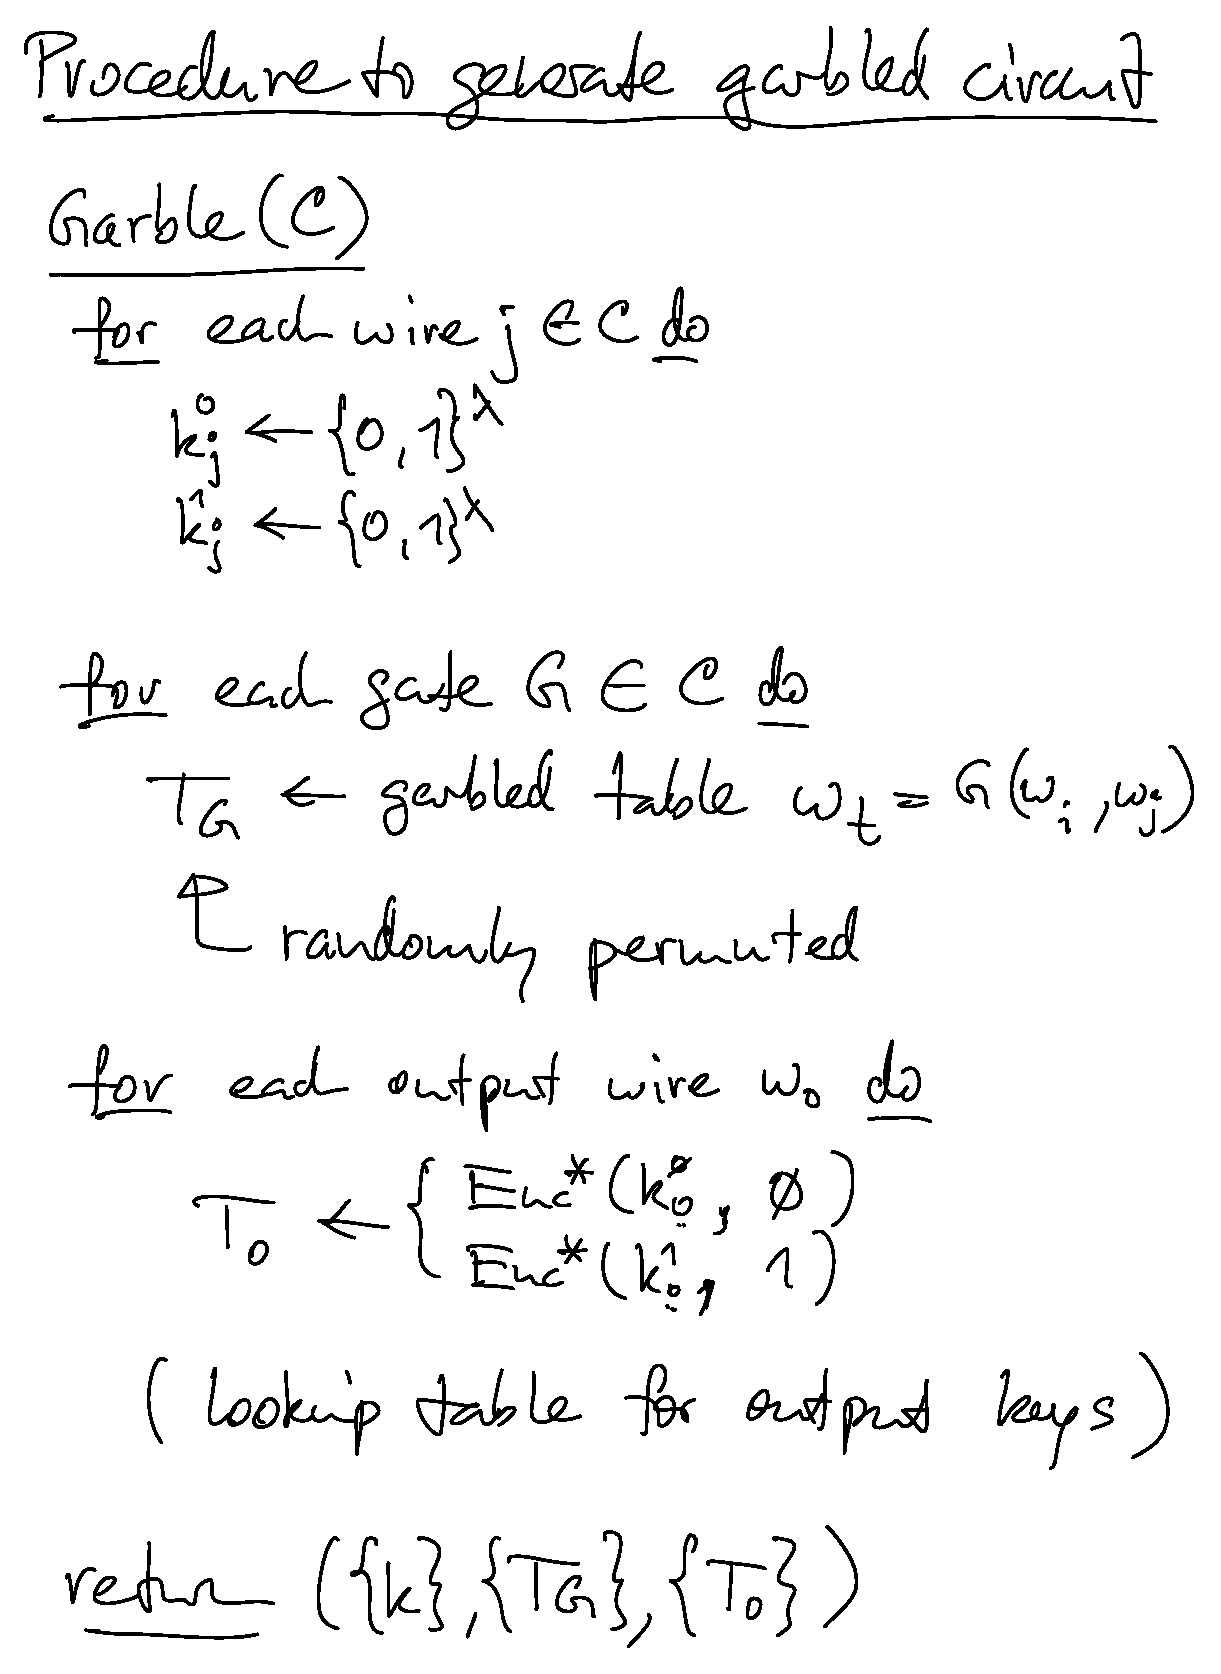
\includegraphics[width=0.7\textwidth]{8_garble}

\subsubsection{Evaluate garbled circuit}

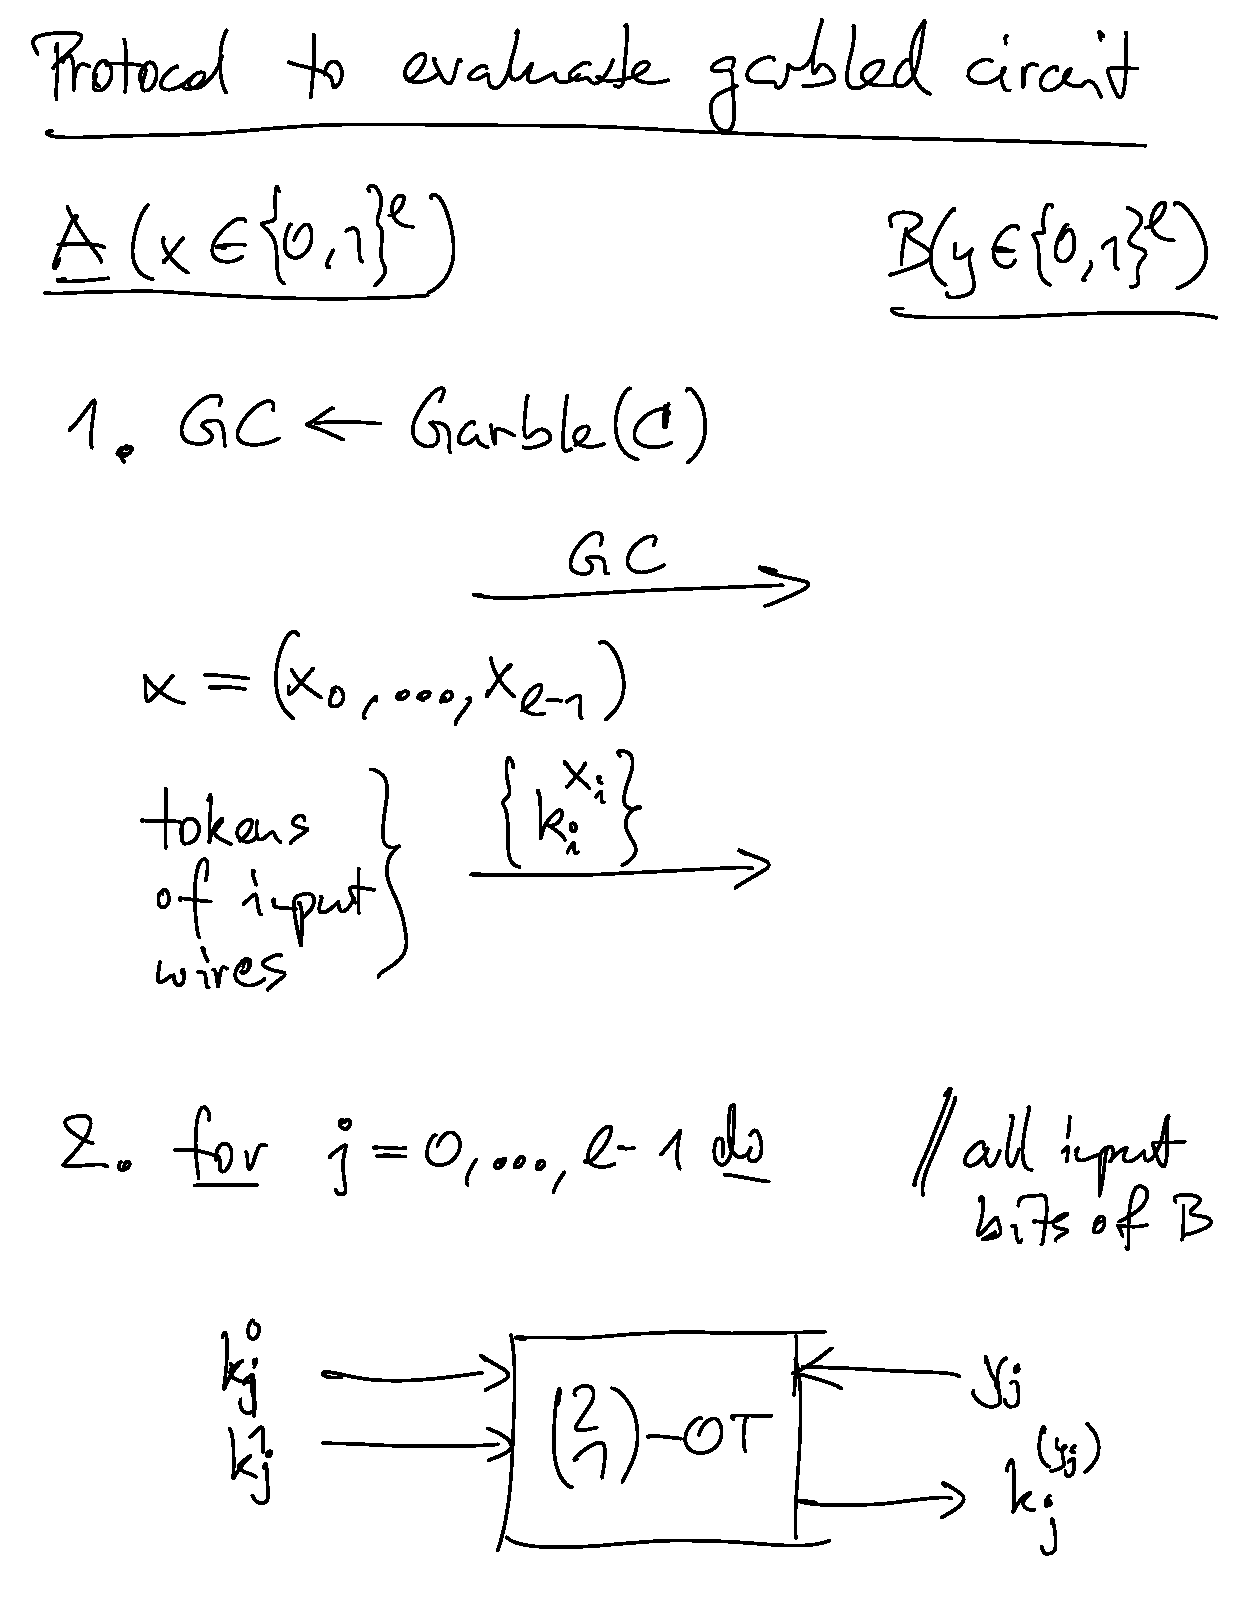
\includegraphics[width=0.7\textwidth]{8_evaluate}

Finally evaluate the garbled circuit, decode the output bits, and output value
$z = f(x, y)$.


\subsection{Modular protocol for 2PC (GMW protocol)}

Yao's protocol uses special encryption, and does not generalize to $n > 2$
parties. GMW (Goldreich, MIcali, Wigderson) uses only $\operatorname{XOR}$
operations, and is information-theoretically secure. Uses OT as a black box.

Idea:
\begin{itemize}
		\item Use $2-of-2$ secret sharing for each value on wire in $C$: $x
				\leftrightarrow (r, r \oplus x) = (s_A, S_B)$ where $r \rgets
				\{0, 1\}$, $s_A$ given to $A$, $s_B$ to $B$ are shares of $r$
		\item Use OT to evluate each gate in $C$
\end{itemize}

\subsubsection{Sharing inputs}

\begin{itemize}
		\item Parties $A(x)$, $B(y)$ with $x, y$ of length $l$
		\item Circuit $C$ of $f(x, y)$ consisting of NOT, XOR, AND gates
		\item A: Share inputs: $s^A_j \rgets \{0, 1\}, s^B_j \coloneqq x \oplus
				s^A_j$ for $j = 1 \ldots l$
		\item A: Send all of B's shares $s^B_i$ to $B$
		\item B: Share inputs: $s^A_{j+l} \rgets \{0, 1\}, s^B_{j+l} \coloneqq x \oplus
				s^A_{j+l}$ for $j = 1 \ldots l$
				\begin{itemize}
						\item Note how wire indices shifted, just so we don't
								have an index conflict of shares for inputs of
								$A$ and $B$. Alternative notation would
								introduce third index per share.
				\end{itemize}
		\item $A$ and $B$ now have one share each for all the inputs.
\end{itemize}

\subsubsection{Evaluating XOR gates}

For every gate in $C$ in some topological order, evaluate as follows:

\paragraph{XOR gates}

$w_t = w_i \oplus w_j$, where:
\begin{itemize}
		\item $A$ holds $s^A_i, s^A_j$, $B$ holds $s^B_i, s^B_j$
		\item Such that $s^A_i \oplus s^B_i = w_j$, $s^A_j \oplus s^B_j = w_j$
\end{itemize}

Now:
\begin{align*}
		w_t & = w_i \oplus w_j \\
			& = (s^A_i \oplus s^B_i) \oplus (s^A_j \oplus s^B_j) \\
			& = (s^A_i \oplus s^A_j) \oplus (s^B_i \oplus s^B_j) \\
			& = s^A_t \oplus s^B_t
\end{align*}

So $A$ can compute $s^A_t$, $B$ can compute $s^B_t$ locally, and each now have
a share of the output wire $w_t$.

\paragraph{NOT gates}

$w_t = \neg w_i$, where:
\begin{itemize}
		\item $A$ has $s^A_i$, $B$ has $s^B_i$
		\item Such that $w_i = s^A_i \oplus s^B_i$
\end{itemize}

Now:
\begin{itemize}
		\item $A$ sets $w^A_t \coloneqq s^A_i \oplus 1$
		\item $B$ sets $w^B_t \coloneqq s^B_i$
\end{itemize}

Then $w_t = w^A_t \oplus w^B_t$, so both have a valid share again using only
local operations.

\paragraph{AND gates}

$w_t = w_i \land w_j$, where:
\begin{itemize}
		\item $A$ holds $s^A_i, s^A_j$, $B$ holds $s^B_i, s^B_j$
		\item Such that $s^A_i \oplus s^B_i = w_j$, $s^A_j \oplus s^B_j = w_j$
\end{itemize}

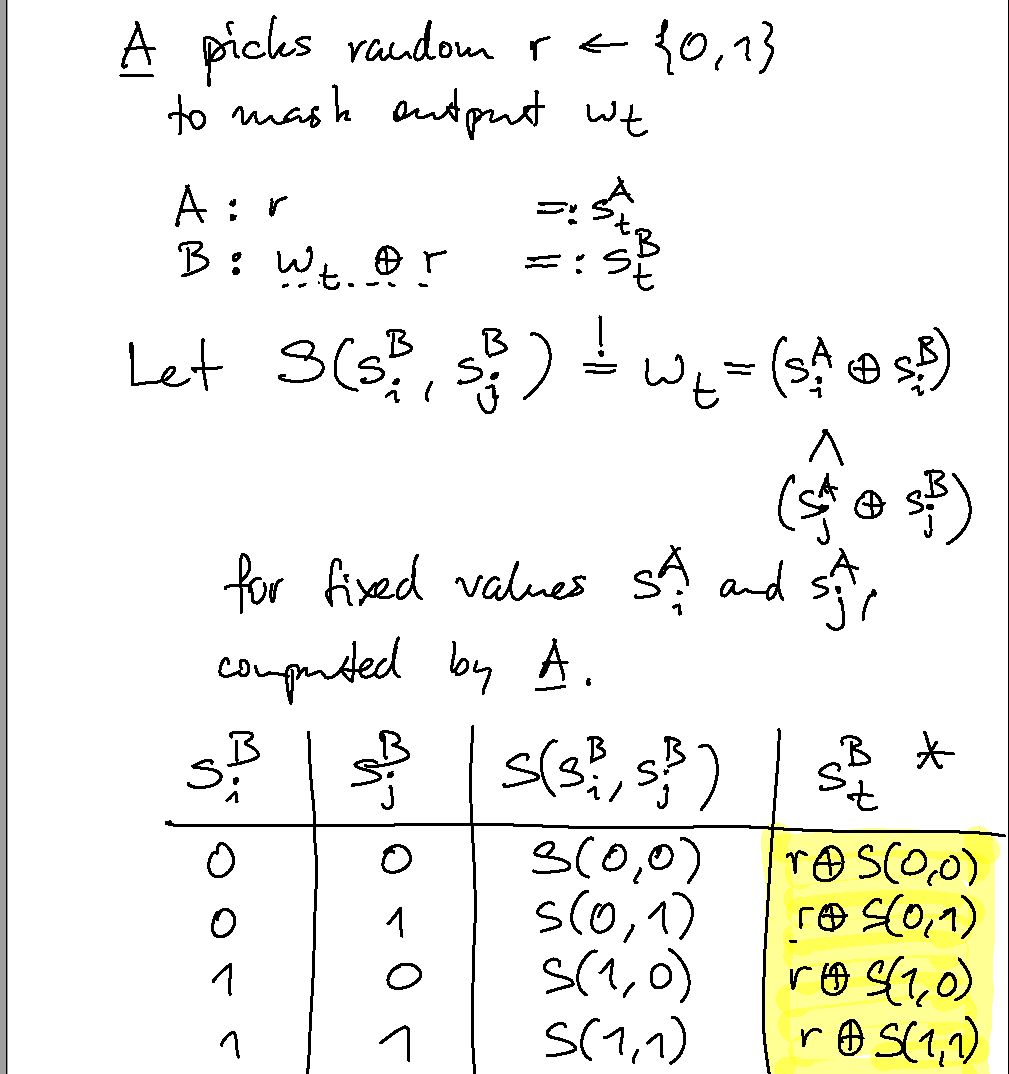
\includegraphics[width=0.7\textwidth]{9_and_1}

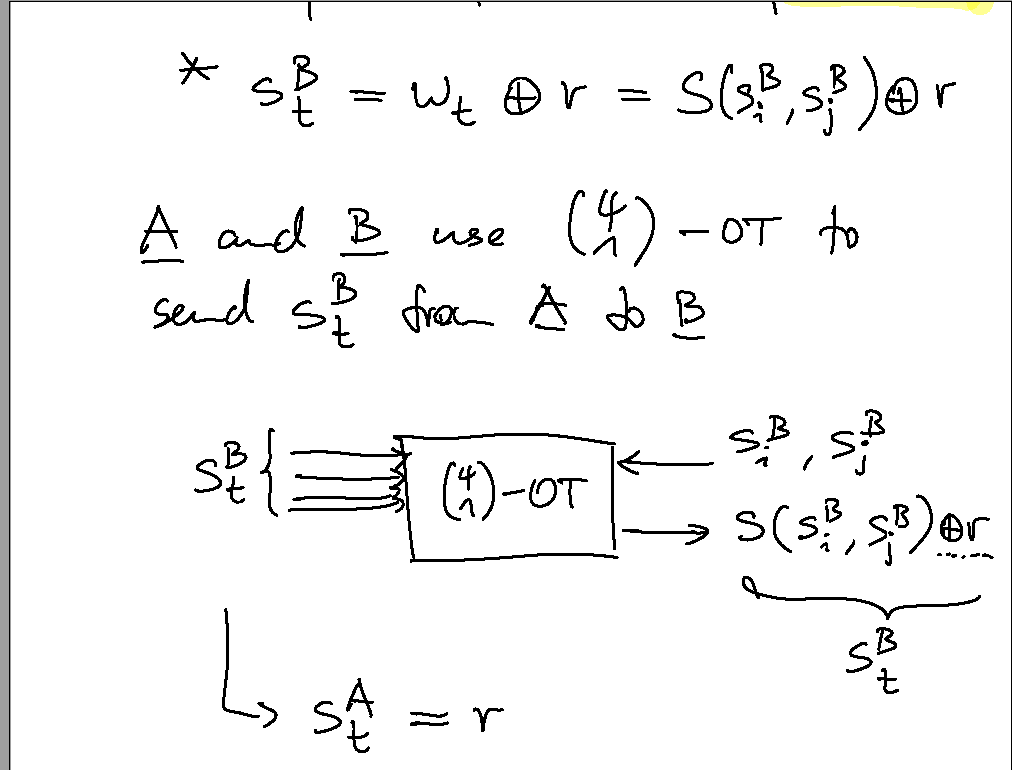
\includegraphics[width=0.7\textwidth]{9_and_2}

\paragraph{Output wires}

\begin{itemize}
		\item A: send ${s^A_o}$ for every output wire $o$ to $B$.
		\item B: $w_o \coloneqq s^A_o \oplus s^B_o$
		\item B: send ${s^B_o}$ for every output wire $o$ to $B$.
		\item A: $w_o \coloneqq s^A_o \oplus s^B_o$
\end{itemize}

Now $A$, $B$ have both reconstructed the values of the output wires.

\paragraph{Cost}

\begin{description}
		\item[Pk-Operations] $O(|C|)$
		\item[Communication bits] $O(|C|)$
		\item[Latency] $O(depth(C))$, higher than Yao's.
\end{description}

Depth is longest path from any input to an output, counting AND gates.

\subsection{Generalisation to $n$ parties $P_1, \ldots P_n$}

Idea: Use additive sharing of secret in $n-out-of-n$ model, $x \leftrightarrow
(x_1, \ldots x_n)$, with $x_i$ given to $P_i$.

Then $w_i$ on wire $i$ is represented by shares $s_1, \ldots, s_n$: $w_i
\leftrightarrow (s^1_i, \ldots, s^n_i)$

Protocol as before, except for AND gates. There:
\begin{align*}
		w_t & = w_i \land w_j \\
			& = (\oplus_{k=1}^n s^k_i) \land (\oplus_{k=1}^n s^k_j) \\
			& = (\oplus_{k=1}^n s^k_i \land s^k_j) \oplus (\oplus_{k, l = 1, k \neq l}^n s^k_i \land s^l_j) \\
\end{align*}

Note how first $\oplus$ operation is those with same lower index, second one
all those with differing ones.

\begin{itemize}
		\item $P_k$ can compute $s^k_i \land s^k_j$ locally
		\item $P_k, P_l$ can compute a 2-of-2-sharing of $s^k_i \land s^l_j$
				using 2-party protocol step with a $4-1 OT$ as before
		\item In the end, $P_1, \ldots, P_n$ again have additive shares of $w_t \leftrightarrow (s^1_t, \ldots s^n_t)$
		\item Using $n \cdot (n - 1)$ OT protocols
\end{itemize}

\section{Distributed cryptography}

Idea: Cryptography with e.g $n = 9$, $t = 4$, secure as long as no more than
$t$ of the parties are corrupted.

\subsection{Secret sharing}

Share secret $s$ among parties $P_1, \ldots, \P_n$ such that any $t+1$ parties
can recover it, and no $t$ (or fewer) parties have any information on $s$.

\begin{itemize}
		\item Dealer picks random polynomial $f(x)$ over $GF(q)$ of degree $t$,
				such that $f(0) = s$: $f(x) = \sum_{i=1}^t f_i \cdot x^i + s$
		\item D gives $s_i = f(i)$ to $P_i$
		\item From any $t+1$ points, the polynomial, and therefore $s = f(0)$, can be recovered
\end{itemize}


\subsection{Threshold ElGamal}

Idea: Encrypt such that any $f+1$ clients together can decrypt the ciphertext.
For key generation, have trusted party distribute shares of private key $x
\leftrightarrow (x_1, \ldots, x_n$) using $f+1$-out-of-$n$ secret sharing.

For encryption, regular hashed ElGamal, $R \coloneqq g^r, C \coloneqq H(y^r)
\oplus m$.

For decryption:
\begin{itemize}
		\item Client sends $(R, C)$ to all parties $P_1, \ldots, P_n$
		\item Party $P_i$ computes $d_i \coloneqq R^{x_i}$ and sends to client
		\item Having received $f+1$ decryption shares, the client computes $z
				\coloneqq \prod d_i^{\lambda^s_{0,i}}$. Now $z = y^r$, so it
				computes $\hat{m} \coloneqq H(z) \oplus C$ and $\hat{m} = m$
\end{itemize}

Secure against passive attacks due to properties of secret sharing scheme. Not
robust against malicious parties, as they can release incorrect decryption
shares.

\subsubsection{Robustness against malicious parties}

Dealer generates $y = g^x$ and $y_i = g^{x_i}$ for every party $P_i$. $y_i$ is
publicly released. Then, every party $P_i$ has to additionally prove --- using
a ZKPK --- that it knows the $x_i$ such that $y_i = g^{x_i} \land d_i =
R^{x_i}$.

\subsection{RSA threshold signatures}

Recall: RSA does have a group homomorphism, but we cannot use it as $\varphi(N)$
must not be public. Instead, use $n$-of-$n$ secret sharing over the integers.

\subsubsection{Key generation}

To share secret key $d$, choose random $d_i \rgets [0, N \cdot 2^\lambda]$ such
that $\sum d_i \equiv d \pmod{\varphi(N)}$, with $\lambda = 128$.


\subsubsection{Distributed signature generation}

\begin{itemize}
		\item Every party computes and sends a signature share $\sigma_i
				\coloneqq H(m)^{d_i} \mod N$ to client.
		\item Upon having received $n$ shares, client computes $\sigma
				\coloneqq \prod \sigma_i \mod N$
\end{itemize}


\subsubsection{Impracticality}

Issues:
\begin{itemize}
		\item Only supports $n$-out-of-$n$ secret sharing
		\item Other schemes exist for $f+1$-out-of-$n$ RSA signatures
\end{itemize}

\subsection{Proactive security}

Issue: Over long time, shares are bound to be compromised. Once more than $f$
shares exposed, security is lost.

Idea: Work in epoch. Once per epoch, reshare the secret. Then, as long as fewer
than $f$ shares are lost per epoch, security holds.

\begin{itemize}
		\item Let $x$ be secret, $a(x) = (x_1, \ldots x_n)$ the current shraing
		\item Let $a'(x) = (x'_1, \ldots, x'_n)$ be a new sharing, that is
				$a(0) = a'(0)$. How to generate $a'$ in distributed way?

		\item Each $P_i$ generates a random sharing $b_i(x)$ of $0$, and sends
				the share $b_i(j)$ to every party $P_j$
		\item Then each $P_i$ calculates $x'_i \coloneqq \sum b_j(i) + x_i$
		\item Now, $x'_i$ will be a share for $a'(x)$.
\end{itemize}


\section{Secure multiparty computation (MPC)}

So far we used boolean circuits. Now: Arithmetic circuits over a finite field
$GF(q)$ with $+$ and $\cdot$ operations.

\subsection{Theorem}

For every function $f : \{0, 1\}^* \rightarrow \{0, 1\}$ computed by a boolean
circuit $C_B$, there exists an arithmetic circuit $C_A$ which also computes
$f$. The size of $C_A$ is proportional to the one of $C_B$.

\subsection{BGW protocol: MPC with unconditional security}

Recall GMW protocol for 2PC with unconditional security. Overview of MPC:
\begin{itemize}
  \item Use $f+1$-of-$n$ secret sharing for all wires: $w \leftrightarrow (w_1,
    \ldots, w_n) = [w]$
  \item Implement each gate of circuit
  \item To provide inputs, $P_i$ shares its input $x_i \leftrightarrow
    (x_{i,1}, \ldots, x_{i, n})$
  \item To obtain output, each party releases its share of output
  \item Communication assumes secure channels between all parties, and a
    broadcast channel
  \item Semi-honest model with up to $f$ honest-but-curious
\end{itemize}

\subsubsection{Share input values}

\begin{itemize}
  \item $P_i$ shares $x_i \leftrightarrow (x_{i,1}, \ldots, x_{i, n})$
  \item For each wire $w_i$, parties hold $[w_i]$
\end{itemize}

Notation: $[w_i] = [w_{i, 1}, \ldots, w_{i, n}$, with $w_{i, j} = a_i(j)$.
($j$'s share of wire $i$).

\subsubsection{Evaluate gates}

Using a topological order

\paragraph{Addition gate}

Goal: $[w_t] = [w_j] + [w_k]$

\begin{align*}
  [w_t] & = [w_j] + [w_k] \\
        & = (a_j(1), \ldots, a_j(n)) + (a_k(1), \ldots, a_k(n)) \\
        & = (a_j(1) + a_k(1), \ldots, a_j(n) + a_k(n)) \\
        & = [w_j + w_k]
\end{align*}

Fully local operations, then each party has its share of $[w_j + w_k]$.

\paragraph{Multiplication-by-constant gate}

Goal: $[w_t] = \gamma \cdot [w_j]$.

\begin{align*}
  [w_t] & = \gamma \cdot [w_j] \\
        & = \gamma \cdot (w_{j, 1}, \ldots, w_{j, n}) \\
        & = (\gamma \cdot w_{j, 1}, \ldots, \gamma \cdot w_{j, n}) \\
        & = [\gamma \cdot w_j]
\end{align*}

Again fully local operations.

\paragraph{Multiplication gate}

Goal: $[w_t] = [w_j \cdot w_k]$.

$P_i$ first locally computes $h_{t,i} = w_{j, i} \cdot w_{k, i}$. Notice now
that $h_{t,1}, \ldots, h_{t, n}$ define a polynomial $b_t(x)$ such that $b_t(i)
= h_{t, i} = w_{j, i} \cdot w_{k, i} = a_j(i) \cdot a_k(i)$ has degree $2f$.

Observe that $b_t(0) = a_j(0) \cdot a_k(0) = w_j \cdot w_k = w_t$. That is it
is a valid sharing of the output wire, but with too high a degree. Issue:
Chained multiplication gates would cause degree to escalate.

There exist lagrange coefficients such that $w_t = b_t(0) = \sum_{i=1}^{2f + 1}
\lambda_i \cdot b_t(i)$.

This is evaluated using another `shared' computation:
\begin{itemize}
  \item $P_i$ shares $h_{t, i} \leftrightarrow (h_{t, i, 1}, \ldots, h_{t, i, n})$
  \item Parties now hold $[h_{t, 1}], \ldots, [h_{t, n}]$
  \item Parties locally compute $[w_t] = \sum_{i=1}^{2f+1} \lambda_i \cdot [h_{t, i}] = [\sum_{i=1}^{2f + 1} \lambda_i \cdot h_{t_i}]$
  \item This now is a new $f+1$-of-$n$ sharing of $w_t$
\end{itemize}

\paragraph{Output reconstruction}

\begin{itemize}
  \item For each output wire $o$, parties hold $[w_0]$.
  \item $P_i$ broadcasts its share $w_{o, i}$
  \item $P_i$ receives enough shares to reconstruct $w_o$
\end{itemize}

\paragraph{Cost}

\begin{description}
  \item[Public-key operations] $O$ (unconditional)
  \item[Communication bits] $O(|C| \cdot n^2)$
  \item[Communication rounds] $O(depth(C))$
\end{description}


\end{document}

